\documentclass[10pt, a4paper]{article}

\usepackage{listings}
\usepackage{graphicx}
\usepackage[top=1.5in, bottom=1.5in, left=1in, right=1in]{geometry}
\begin{document}

\title{CS22510 Assignment}
\author{Samuel B Sherar (sbs1)}

\maketitle

\newpage

\tableofcontents

\newpage

\section{Event Creation}

\subsection{Code}
\lstset{tabsize=2, breaklines=true, breakatwhitespace=true, basicstyle=\ttfamily}
\subsubsection{main.cpp}
\lstinputlisting{../event-creation/main.cpp}

\subsubsection{CLI.h}
\lstinputlisting{../event-creation/CLI.h}

\subsubsection{CLI.cpp}
\lstinputlisting{../event-creation/CLI.cpp}

\subsubsection{Competitors.h}
\lstinputlisting{../event-creation/Competitors.h}

\subsubsection{Competitor.cpp}
\lstinputlisting{../event-creation/Competitor.cpp}

\subsubsection{List.h}
\lstinputlisting{../event-creation/List.h}

\subsubsection{Course.cpp}
\lstinputlisting{../event-creation/Course.cpp}

\subsubsection{Event.h}
\lstinputlisting{../event-creation/Event.h}

\subsubsection{Event.cpp}
\lstinputlisting{../event-creation/Event.cpp}

\subsubsection{FileWriter.h}
\lstinputlisting{../event-creation/FileWriter.h}

\subsubsection{FileWriter.cpp}
\lstinputlisting{../event-creation/FileWriter.cpp}

\subsubsection{Makefile}
\lstinputlisting{../event-creation/Makefile}


\subsection{Compiler Output}
\begin{lstlisting}
event-creation(master*): make clean && make
rm -rf bin/*
g++ -g -Wall main.cpp Event.cpp Course.cpp Competitor.cpp CLI.cpp FileWriter.cpp -o bin/run

\end{lstlisting}

\subsection{Terminal Output}
\lstinputlisting{output/event-creation.txt}

\subsection{Files Created}

\subsubsection{Event}
\lstinputlisting{../event-creation/data/event.txt}

\subsubsection{Competitors}
\lstinputlisting{../event-creation/data/comp_data.txt}

\subsubsection{Courses}
\lstinputlisting{../event-creation/data/courses.txt}

\newpage

\section{Checkpoint Manager}
\lstset{breakatwhitespace=false}
\subsection{Code}

\subsubsection{uk/co/samsherar/cs22510/Run.java}
\lstinputlisting{../checkpoint-manager/src/uk/co/samsherar/cs22510/Run.java}

\subsubsection{uk/co/samsherar/cs22510/Controller/Manager.java}
\lstinputlisting{../checkpoint-manager/src/uk/co/samsherar/cs22510/Controller/Manager.java}

\subsubsection{uk/co/samsherar/cs22510/Controller/FileParser.java}
\lstinputlisting{../checkpoint-manager/src/uk/co/samsherar/cs22510/Controller/FileParser.java}

\subsubsection{uk/co/samsherar/cs22510/Model/Course.java}
\lstinputlisting{../checkpoint-manager/src/uk/co/samsherar/cs22510/Model/Course.java}

\subsubsection{uk/co/samsherar/cs22510/Model/Entrant.java}
\lstinputlisting{../checkpoint-manager/src/uk/co/samsherar/cs22510/Model/Entrant.java}

\subsubsection{uk/co/samsherar/cs22510/Model/EventInfo.java}
\lstinputlisting{../checkpoint-manager/src/uk/co/samsherar/cs22510/Model/EventInfo.java}

\subsubsection{uk/co/samsherar/cs22510/View/MainFrame.java}
\lstinputlisting{../checkpoint-manager/src/uk/co/samsherar/cs22510/View/MainFrame.java}


\subsection{Compiler Output}
\lstinputlisting{output/checkpoint-manager.txt}

\subsection{Screen Shots}

\subsubsection{No inputs}
\begin{center}
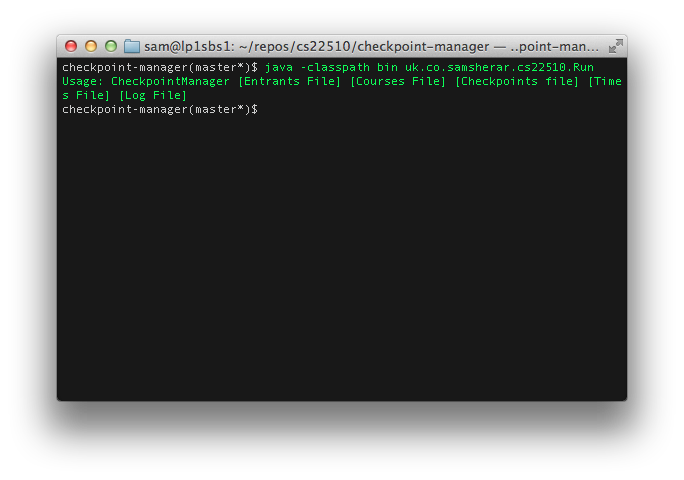
\includegraphics[width=\textwidth]{./screenshots/no-values.png}
\end{center}


\subsubsection{Main GUI}
\begin{center}
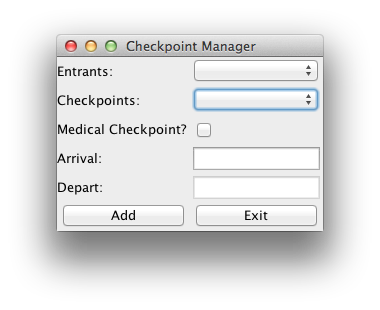
\includegraphics[width=0.5\textwidth]{./screenshots/main-gui.png}
\end{center}

\subsubsection{Medical Checkpoint}
\begin{center}
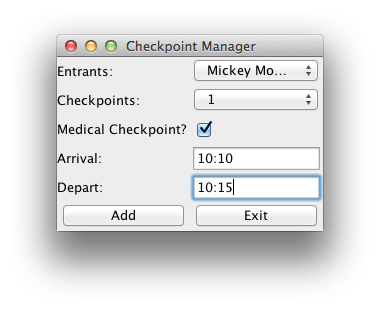
\includegraphics[width=0.5\textwidth]{./screenshots/medical.png}
\end{center}

\subsubsection{Feedback}
\begin{center}
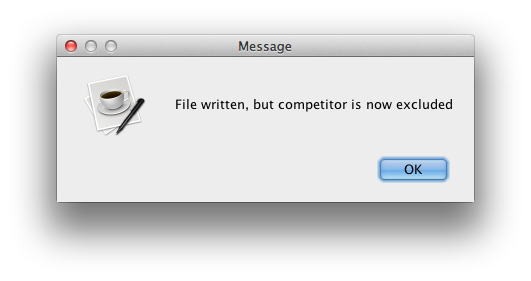
\includegraphics[width=0.75\textwidth]{./screenshots/feedback.png}
\end{center}

\subsubsection{File locking}
\lstinputlisting{./output/file-locking.txt} \footnote{I have used chflags to keep the file locked for the whole time I am needing it, so it's easier for me to test that it is working}

\newpage

\section{Event Manager}

\subsection{Compiler Output}
\lstinputlisting{./output/event-manager.txt}

\subsection{Output Generated \& Results}
\lstinputlisting{./output/event-manager-output.txt}

\subsection{Log File}
\lstinputlisting{../event-manager/data/log.txt}

\section{Descriptions}

\subsection{Event Creator}
For the Event Creator, I decided to use C++. This was because of the great libraries I could use for parsing data on the commandline, while not having to rewrite the Event Manager in a different language. If I were to start from afresh, I would have written the Event Creator in C, mainly because it isn't as powerful as C++. 

I also designed it to use a Model-View-Controller meta-pattern in this program to an extent, so it's easy to edit and modify if/when an update needs to be rolled out. 

\subsection{Event Manager}
For the Event Manager, I decided to not reinvent the wheel and keep it in C. However, I created a new file for the logging and file locking, so there won't be any conflicts with the current code. For the file locking, I have used the example given to us, but with an added method using \verb+ F_GETLK +, which will not set the lock, but returns -1 if there is a lock currently on the file.

\subsection{Checkpoint Manager}
For the Checkpoint Manager, I decided to use Java. This is because I am comfortable creating good GUIs in little time, which will be consistant

I also decided to use the Model-View-Control meta-pattern as it seems the most appropiate for a GUI based application, and it can easily be updated upon in the future. I also have used a Singleton design pattern for the main Controller of the program, which will allow for a single static datasource between all different packages. If the program was any larger, I would have opted for an Observable pattern across, but it seemed a little overpowered for what was needed for this assignment. 

\end{document}
